\documentclass[letterpaper, 11pt]{article} 

\usepackage{graphics,graphicx}
\usepackage{multicol} 
\usepackage{parskip}
\usepackage{amsmath}
\usepackage{multirow}
\usepackage[utf8]{inputenc}
\usepackage{fancyhdr}
\usepackage[title]{appendix}
\usepackage{wasysym}
\usepackage{url}
\usepackage{subcaption}

\usepackage[font=footnotesize,labelfont=small]{caption}
\captionsetup{width=0.85\linewidth}

\RequirePackage{geometry}
\geometry{margin=2cm}

\setlength{\parskip}{0.2cm}
\setlength{\parindent}{0pt}


\title{Assignment 3}
\author{
Tai Duc Nguyen \\
BMES T580: Systems Neuroscience in Medicine and Engineering
}
\date{\today}

\begin{document}

\maketitle

\rule{\textwidth}{1pt}

\section{Problem 1}
\label{sec:prob1}
\textbf{Problem statement:} The figure below shows recordings from two simultaneously recorded cells from a brain region in rats. First column: Food is randomly scattered on the border. Second column: Food is placed at 4equally spaced fixed points as the rat searches the room. Third column: same experiment as first column but after the directed search. Answer the following questions:

a. What kind of recording do you think is being used here?

b. What area of the brain are the researchers recording from? Justify your answer.

c. What elementary computations are necessary to generate cells with these properties?

d. Briefly, describe the neural circuit underlying these computations in the mammalian brain?

\begin{figure}[htb!]
	\centering
	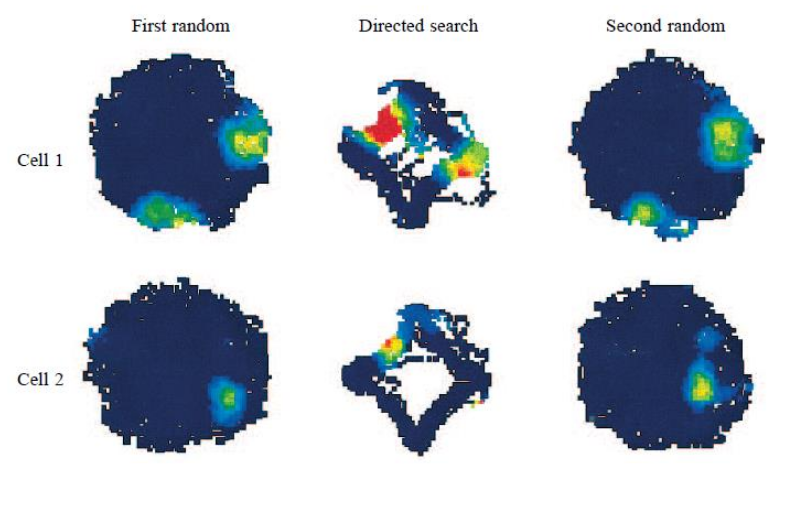
\includegraphics[width=0.8\linewidth]{fig1.png}
	%	\caption{DFF's Layout in Cadence's Virtuoso Layout Suite}
	\label{fig1}
\end{figure}

\textbf{Answer:}

a. From the figure:

\begin{enumerate}
	\item The cell's activation level is being measured
	\item The spatial location of the rat on the field is being recorded
\end{enumerate}

Hence, the researchers likely used the patch-clamp method to record the cell's activities and then map that activity on to the current location of the rat on the field

b. The area of the brain that the researchers get the recording from is the hippocampus because it is where navigation mostly take place. The cell being recorded is likely a place cell

c. These cells have to be able to compute:

\begin{enumerate}
	\item The rat's real world location based on its movement, its direction of movement and a starting location
	\item The characteristic of a piece of food (sensory information)
	\item The likelihood of finding food at a particular location stored in memory (a map)
\end{enumerate}

d. The neural circuits includes: the visual pathway, the inferotemporal cortex, the other sensory pathway, the hippocampus and the prefrontal cortex

The visual pathway is connected to the inferotemporal cortex so that raw visual information of worldly objects is condensed into hierachical representations. These representations are sent to other sensory processing area, the pre-frontal cortex (for decision making), and the hippocampus (for long/short term memory creation and spatial navigation).

\begin{figure}[htb!]
	\centering
	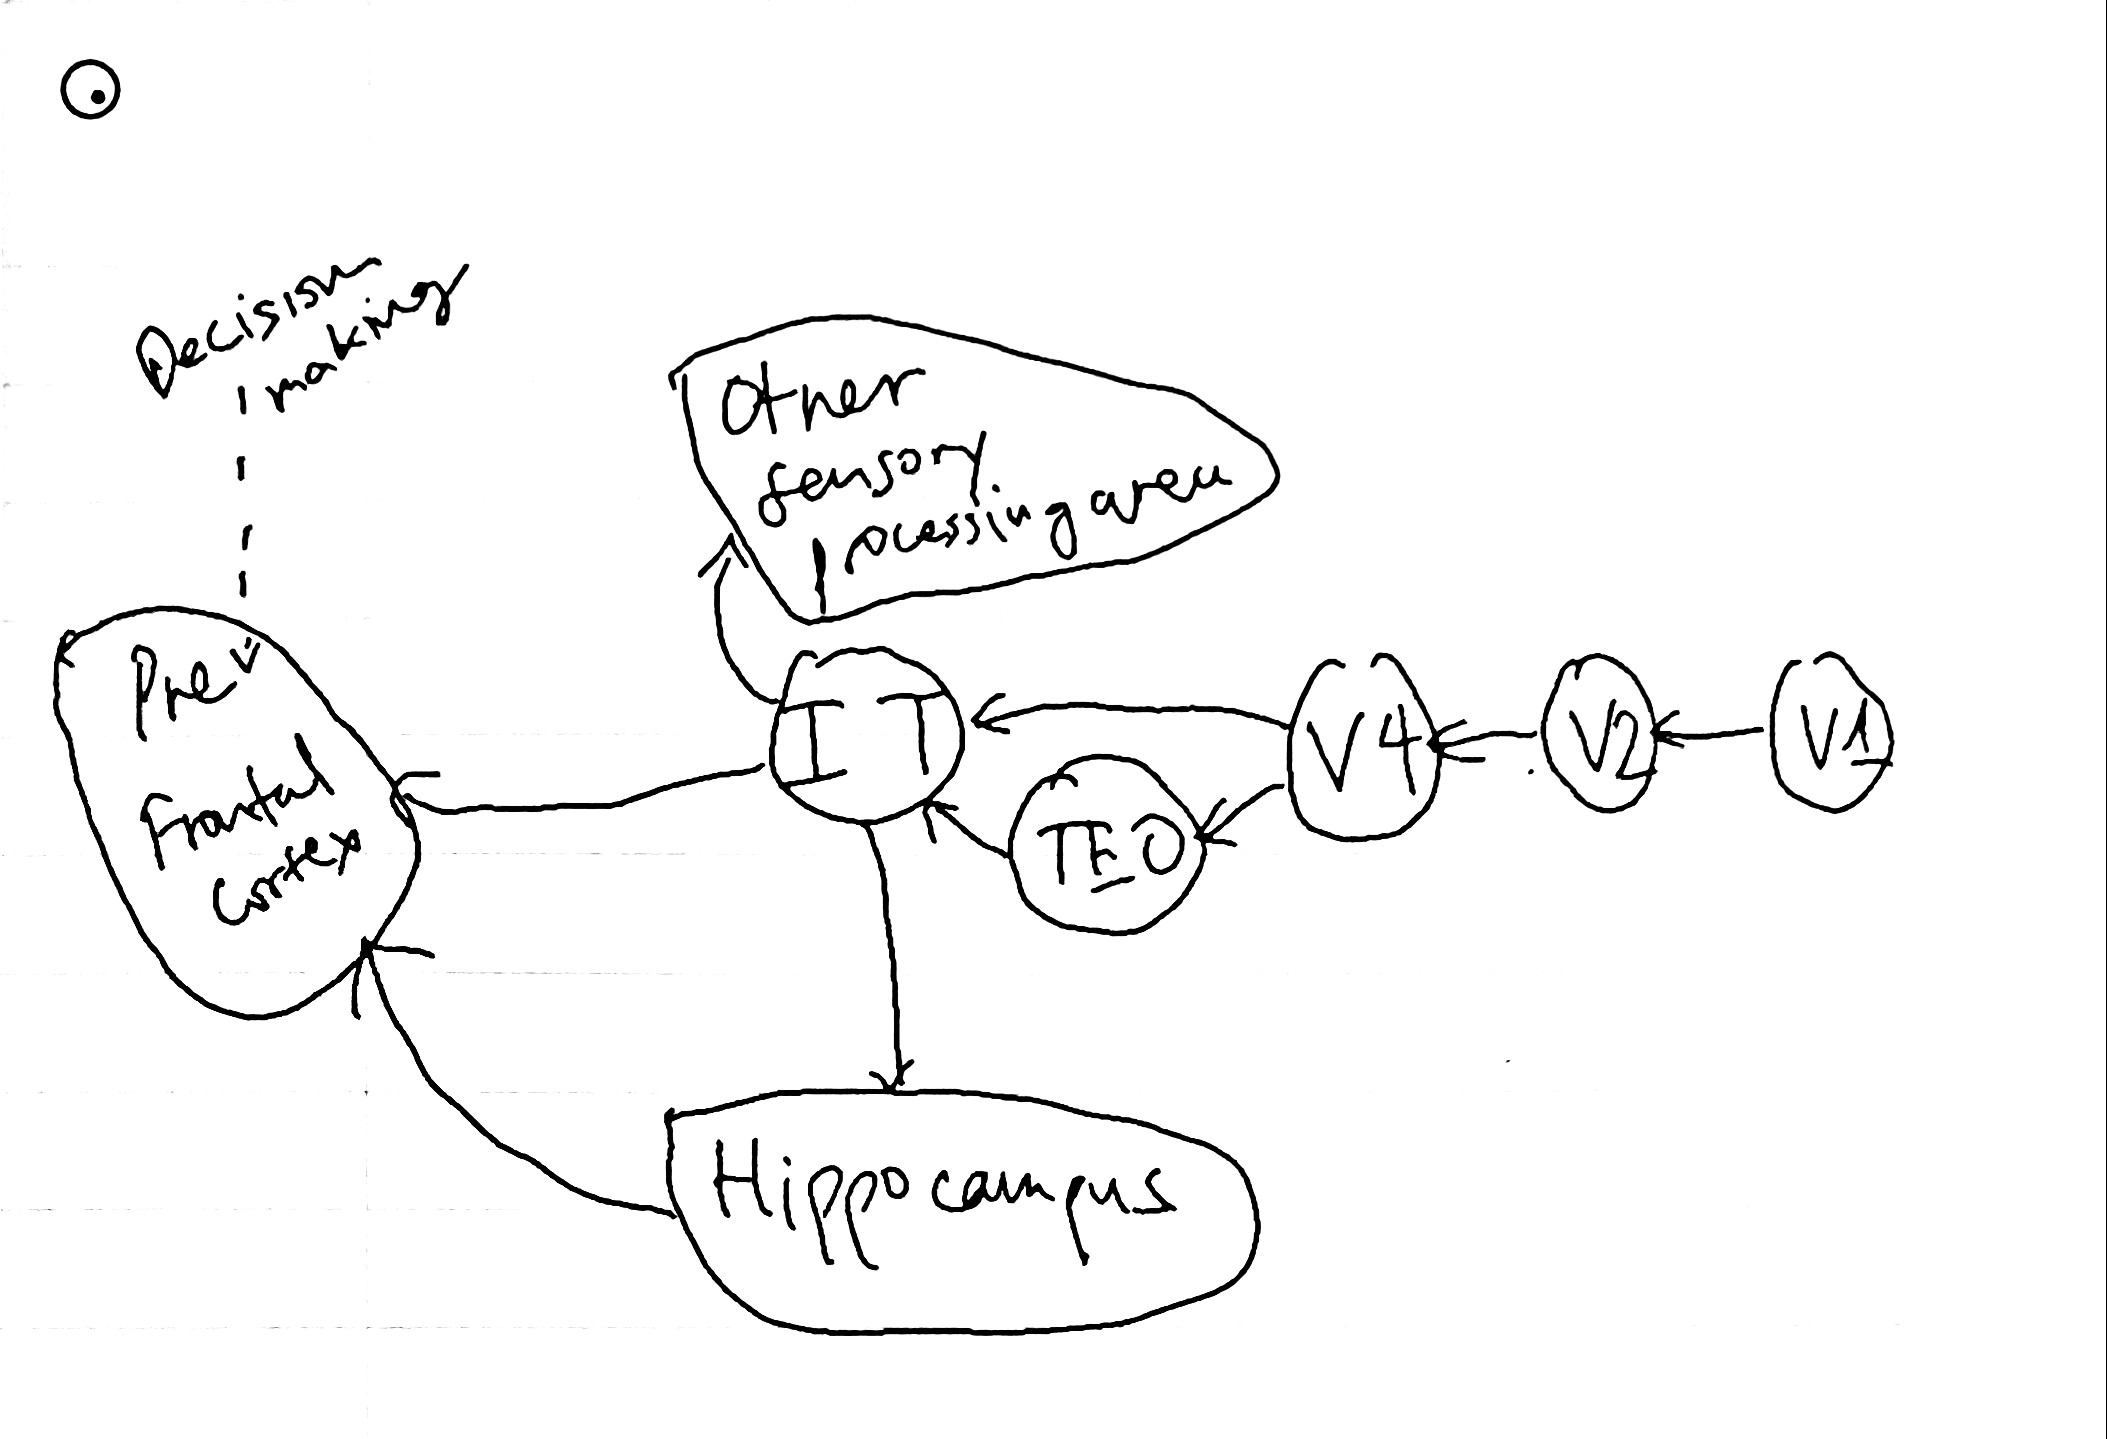
\includegraphics[width=0.8\linewidth]{prob1d.jpg}
	\label{fig1d}
\end{figure}

\section{Problem 2}
\label{sec:prob2}
\textbf{Problem statement:} The figure below shows an experiment (left figure) and the result (right). Answer the following two questions: 

a. What phenomenon is being tested here?

b. What are the possible neural mechanisms that might explain the tested phenomenon?

\begin{figure}[htb!]
	\centering
	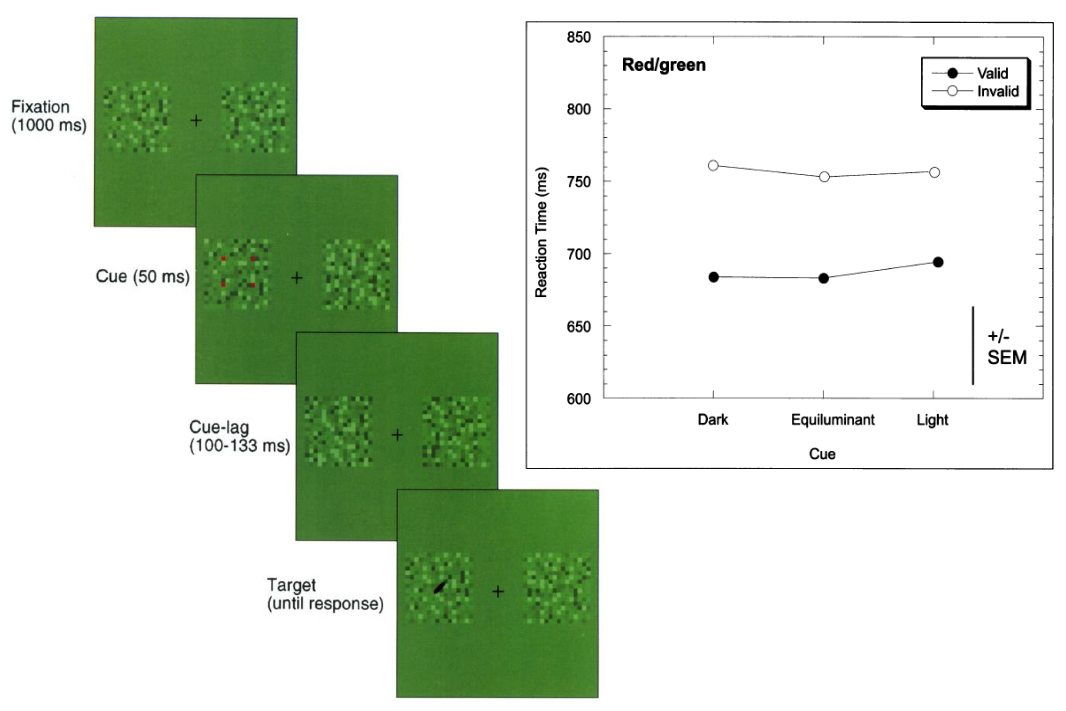
\includegraphics[width=0.7\linewidth]{fig2.png}
	%	\caption{DFF's Layout in Cadence's Virtuoso Layout Suite}
	\label{fig2}
\end{figure}

\textbf{Answer:}

a. It looks like the experiment's aparatus have:

\begin{enumerate}
	\item The participant sitting in front of a screen with a green background
	\item The cue are little red squares (of different contrast) showing on either the left side or the right side
	\item Then the target (in black) appears, which the participant has to press a button to react to the correct location of the target
\end{enumerate}

Hence, it is likely that the researchers are testing if color and color intensity/contrast draws the attention of the participants. The result is that: when the cue is valid, they have a faster response to the target and when the cue is invalid, they have a slower response. Also, the contrast of the little red squares have some, but not major effect on the response to the black target.

b. The possible neural abilities needed for the participant to perform the experiment are:

\begin{enumerate}
	\item The ability to perceive colors
	\item The ability to fixate upon a visual cue
	\item The ability to differentiate the visual cue from the background
	\item The ability to identify the target and response to it
\end{enumerate}

Hence, the neural mechanisms that could explain the phenomenon is that: there are color-sensitive neurons in the visual pathway, which allow the brain to not only discriminate between the background, the clue, and the target but also send signals to other parts of the brain which correspond to attention/fixation. Finally, the decision making part of the brain can also use the color information to response to the target.


\section{Problem 3}
\label{sec:prob3}
\textbf{Problem statement:} The below is a categorization test. Amazingly authors were able to train monkeys to categorize random dot movement pattern in one of 12 directions into 2 categories as shown below.

a. Diagram and describe the experimental paradigm the authors might be employing.

b. Which two areas in the cortex might be involved in this categorization task? Diagram the response pattern of neurons in your chosen area after the monkey’s have learned the categorization.

\begin{figure}[htb!]
	\centering
	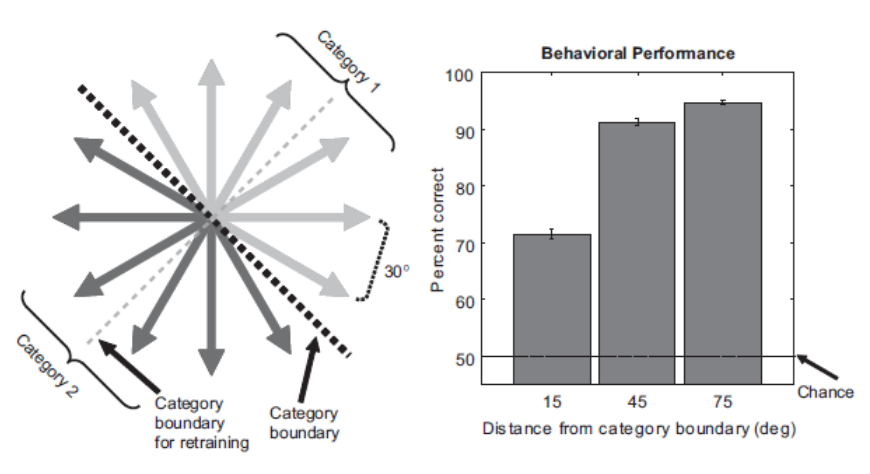
\includegraphics[width=0.8\linewidth]{fig3.png}
	%	\caption{DFF's Layout in Cadence's Virtuoso Layout Suite}
	\label{fig3}
\end{figure}

\textbf{Answer:}

a. In this experiment, the researchers are trying to train monkeys to categorize dot movement of a certain direction. The apparatus may include:

\begin{enumerate}
	\item A monkey in front of a screen
	\item The screen shows a dot starting in the middle, moving away in a certain direction
	\item The monkey has to response to this stimulus by either maintain its grasp or release it (2 categories)
	\item If the monkey got it right, then it is given food as a reward and if it's wrong then it's given nothing
\end{enumerate}

\begin{figure}[htb!]
	\centering
	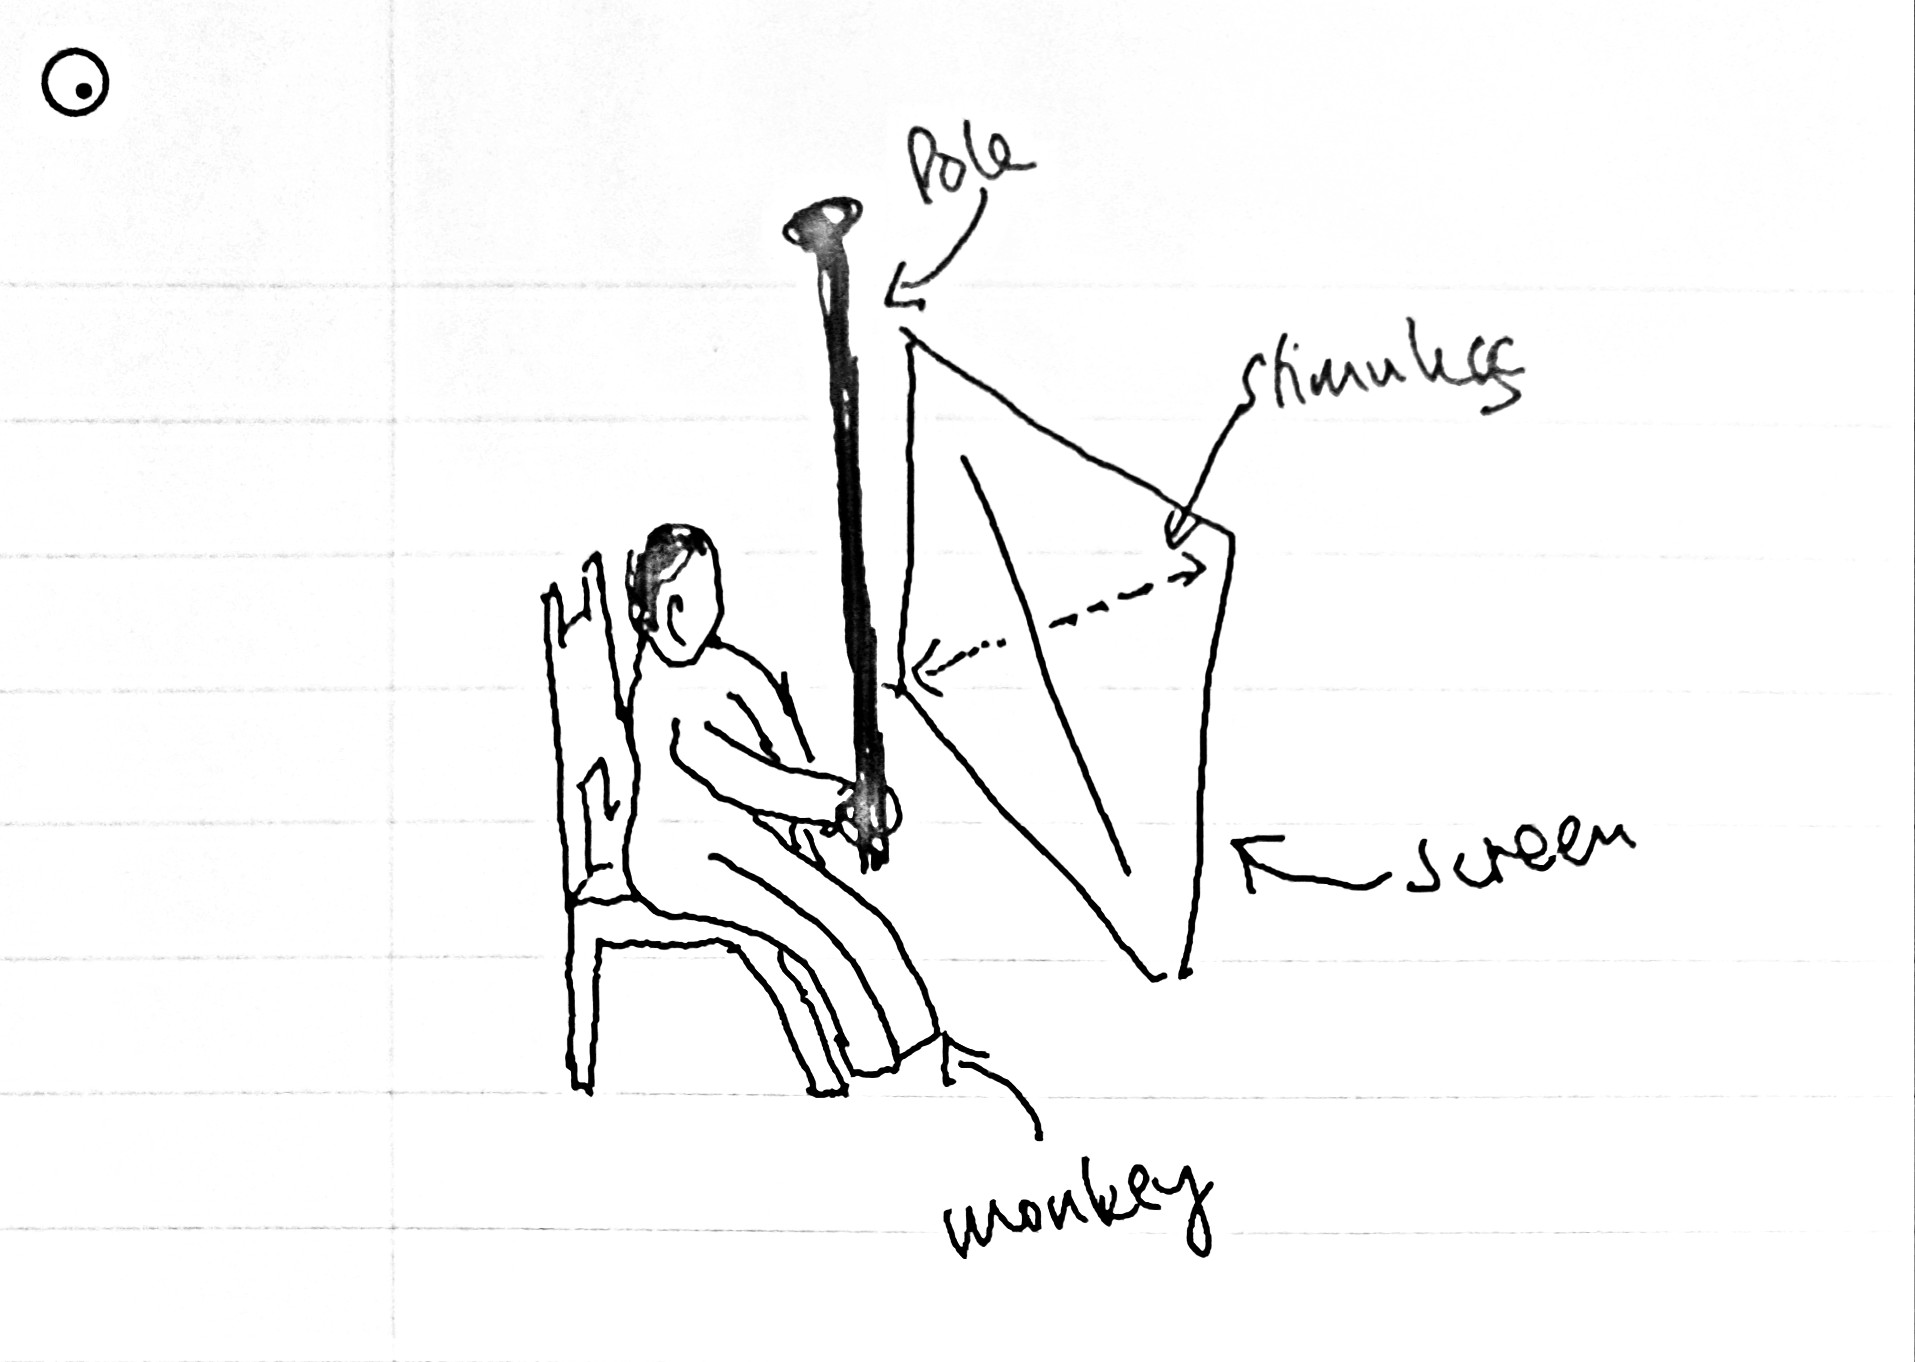
\includegraphics[width=0.6\linewidth]{prob3a.jpg}
	\label{fig3a}
\end{figure}

\newpage

b. The 2 areas in the cortex might be involve in this task is the lateral intraparietal cortex (LIP) and the pre-frontal cortex (PF). The LIP region is notably known for controlling eye saccades, guiding eye movement as in predictive pursuit of an object in space. This region allows the monkeys to track the dot's movement. The PF is known for complex decision making and reinforcement learning.

After training, there would be high correlation (instead of random) in terms of neural activities when the monkey is introduced an input of a certain category


\begin{figure}[htb!]
	\centering
	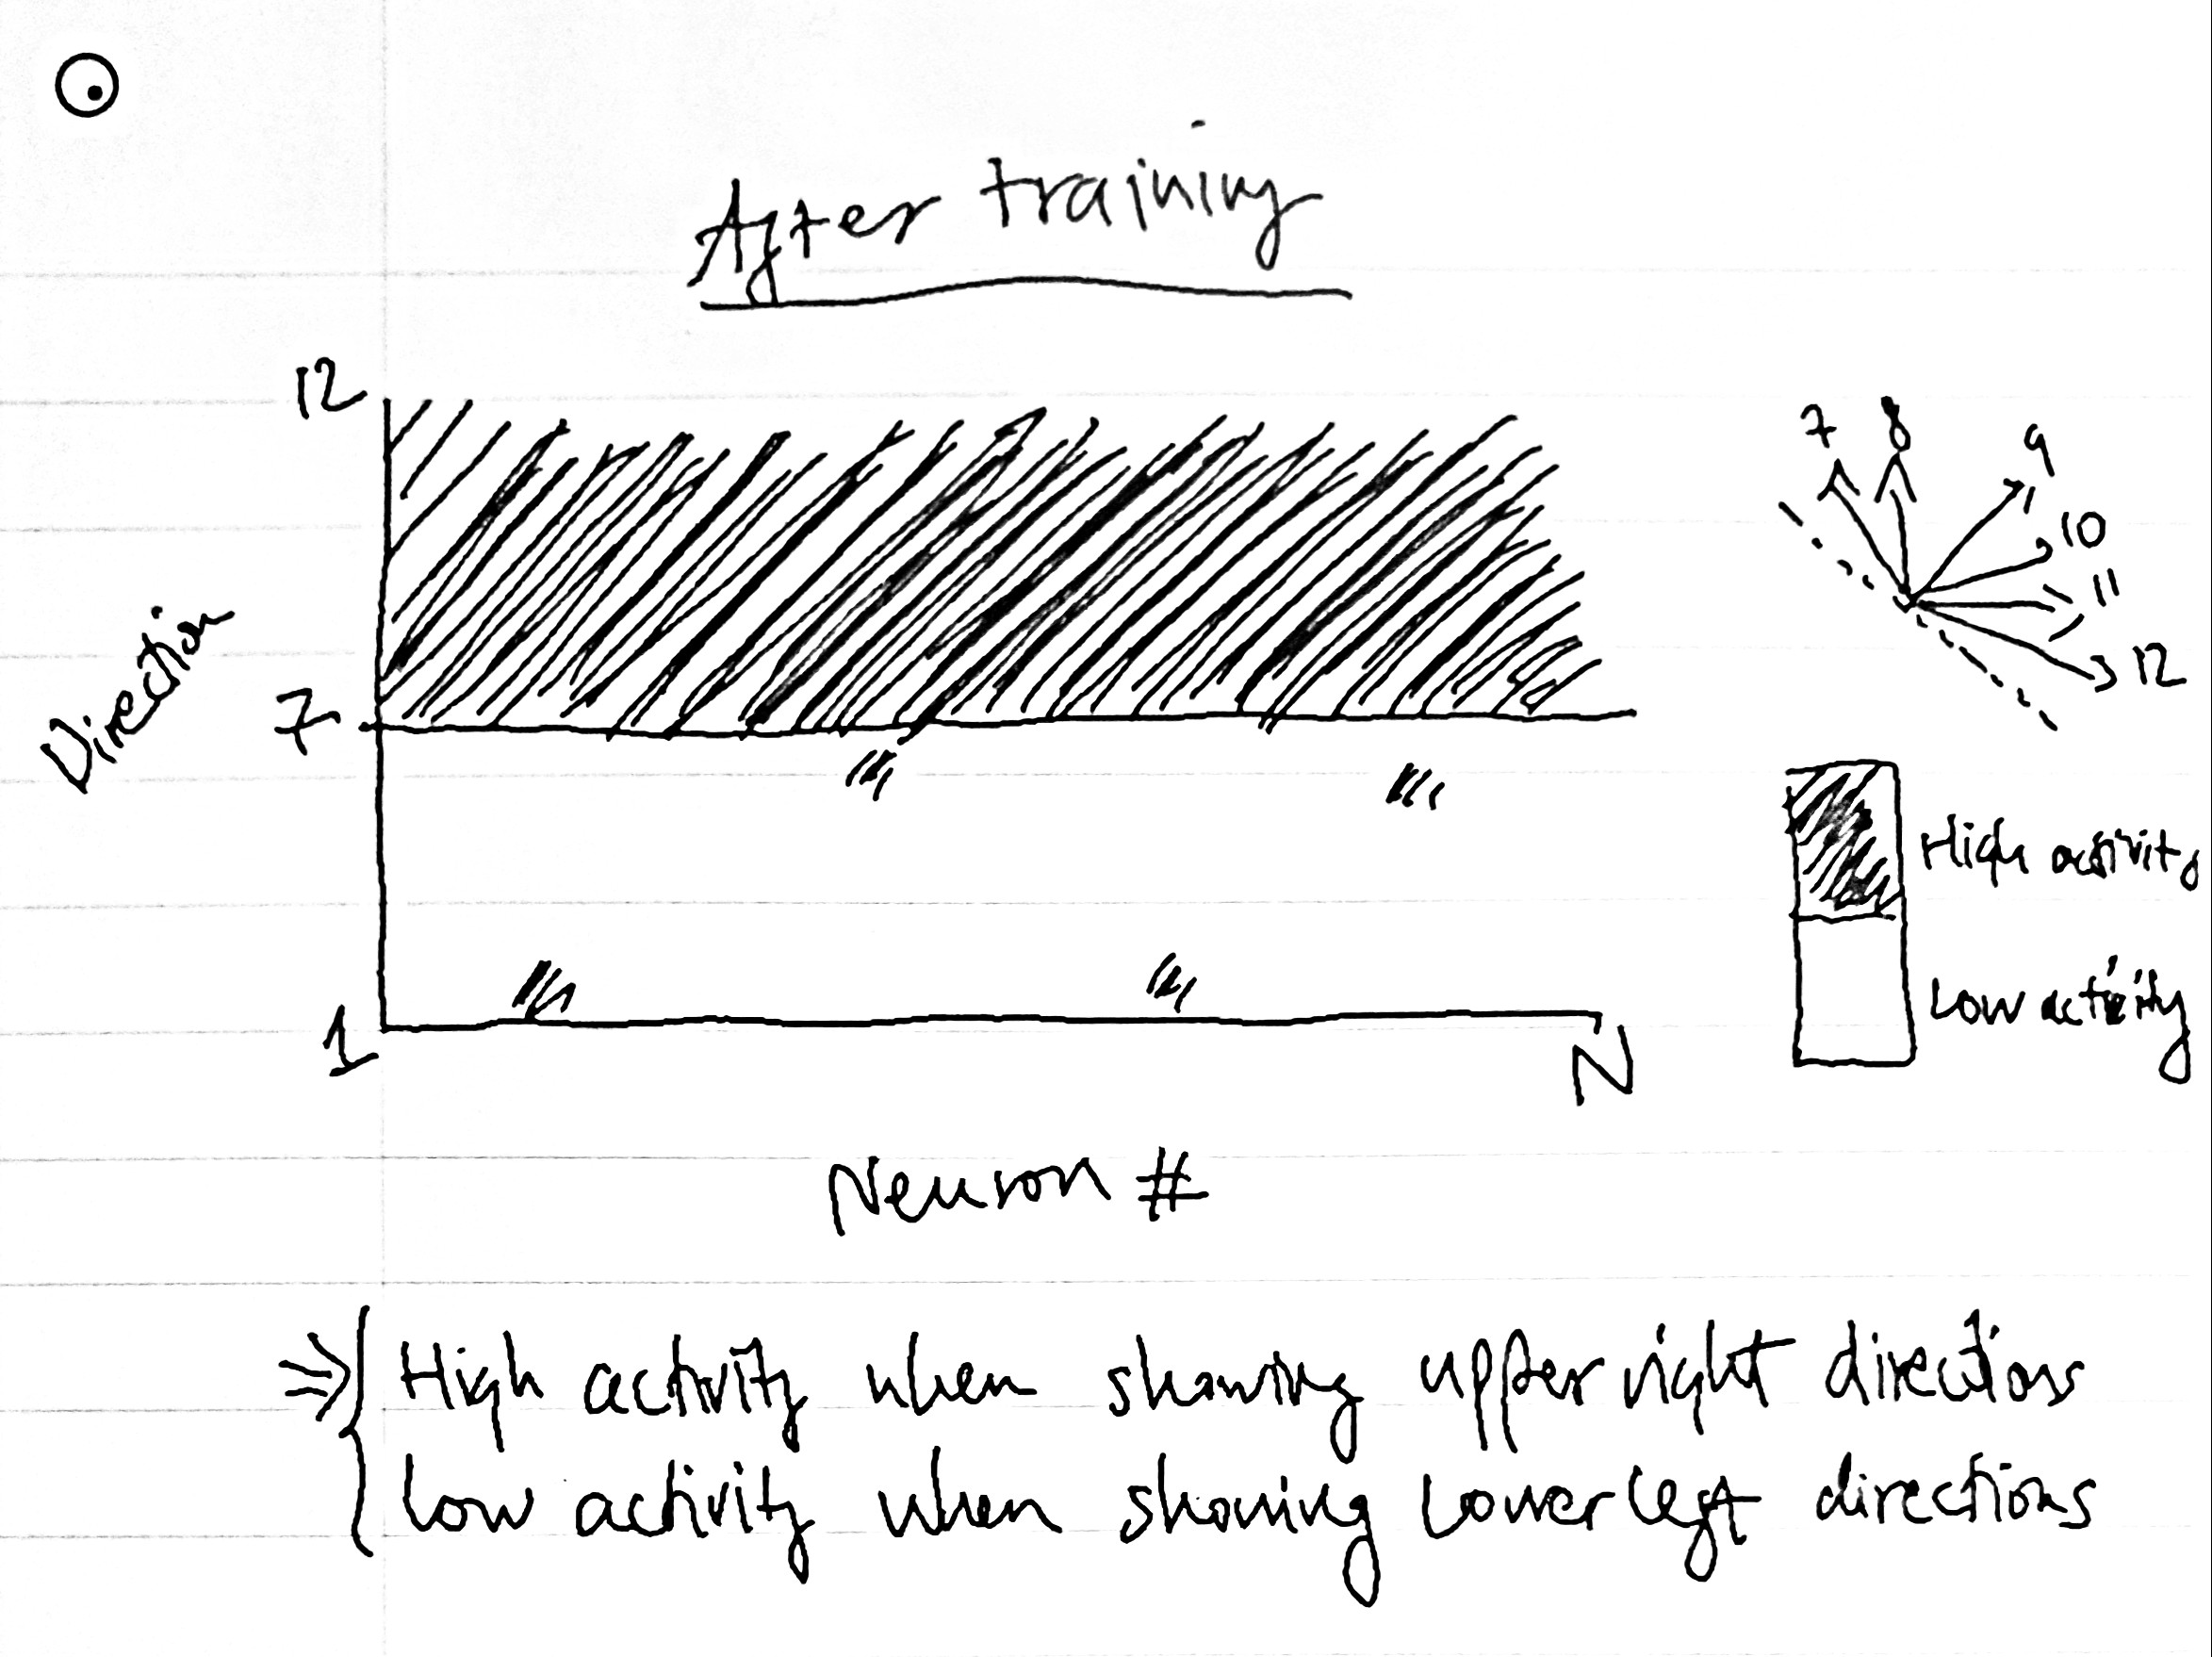
\includegraphics[width=0.8\linewidth]{prob3b.jpg}
	\label{fig3b}
\end{figure}


%\begin{equation}
%Q=\begin{cases}
%1, & \text{Data if rising edge of Clock}.\\
%0, & \text{else keep previous data}
%\end{cases}
%\end{equation}

%\begin{figure}[htb!]
%	\centering
%	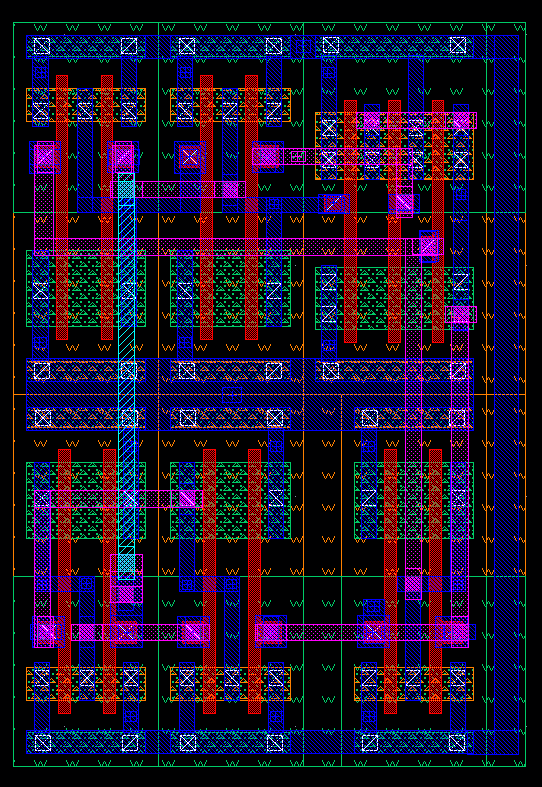
\includegraphics[width=0.6\linewidth]{dff_layout.png}
%	\caption{DFF's Layout in Cadence's Virtuoso Layout Suite}
%	\label{fig8}
%\end{figure}


%\begin{figure}[ht!]
%	\centering
%	\begin{subfigure}[b]{.48\linewidth}
%		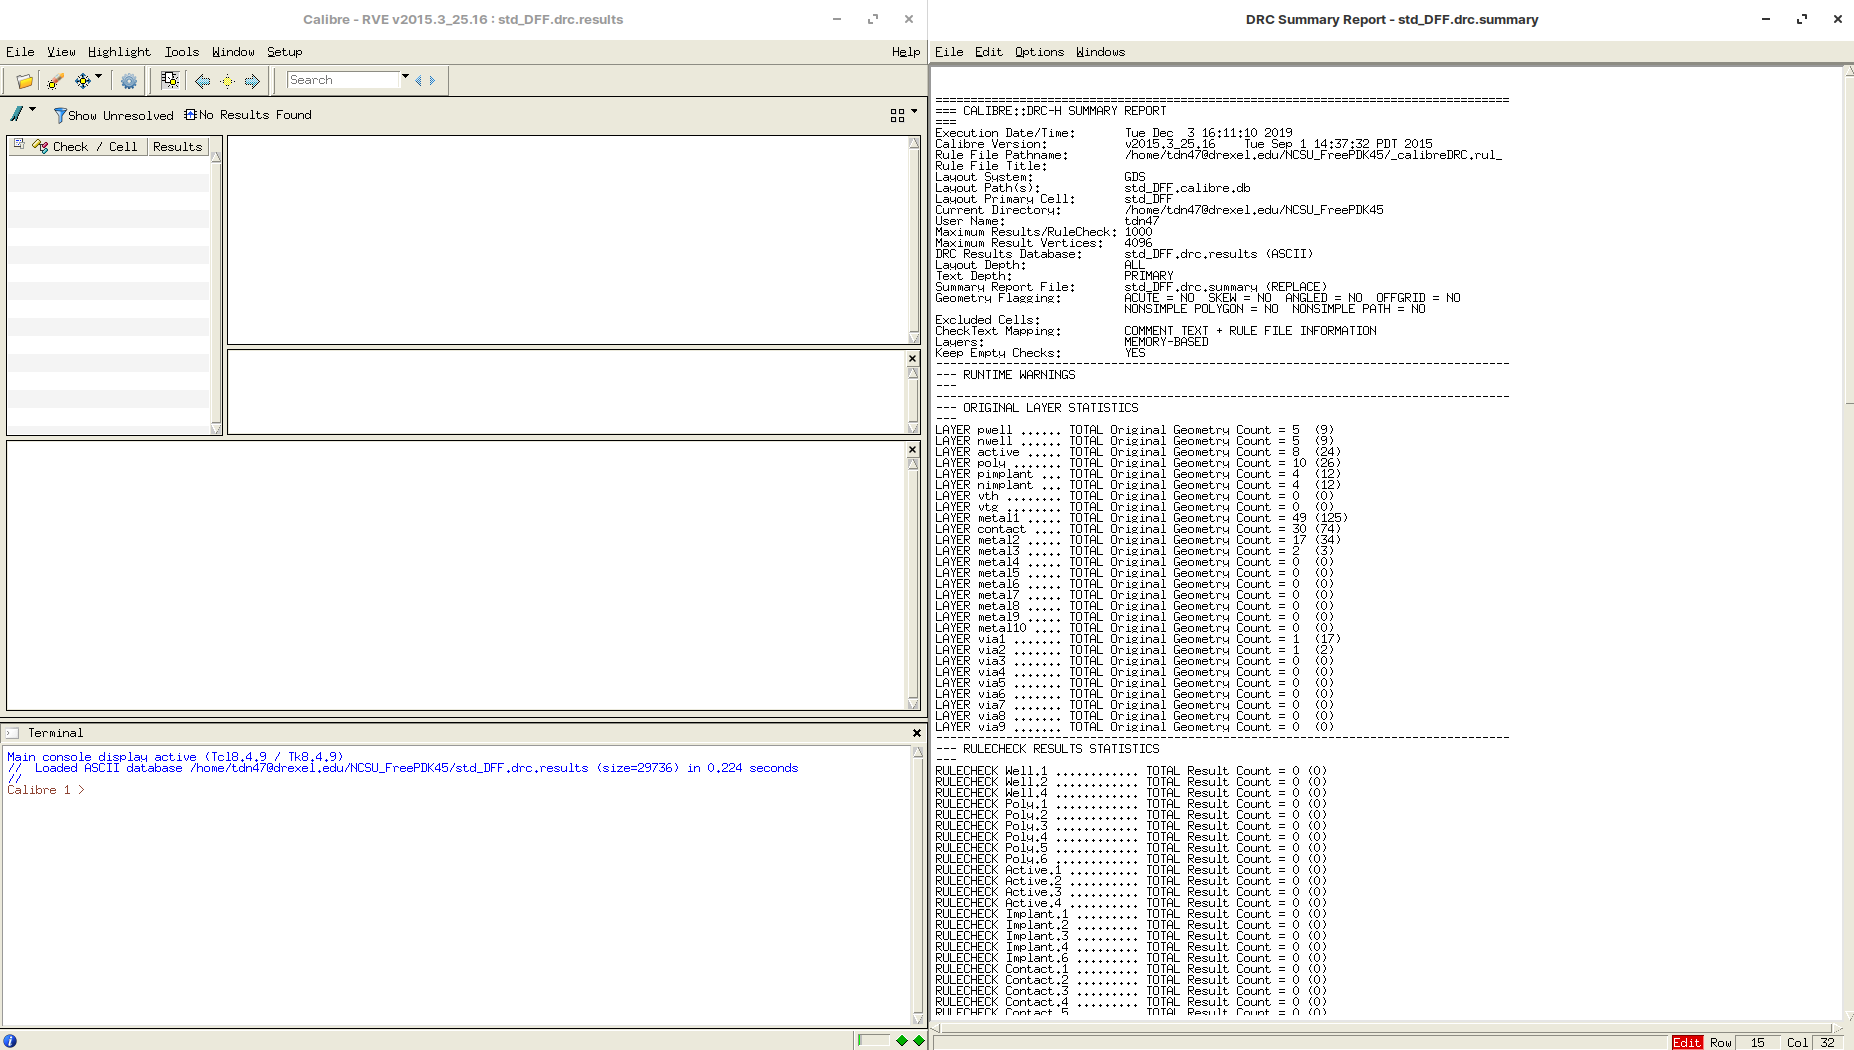
\includegraphics[width=\textwidth]{dff_drc.png}
%		\caption{DFF's rise and fall time}
%		\label{fig9a}
%	\end{subfigure}
%	%	\hskip2em
%	\begin{subfigure}[b]{.48\linewidth}
%		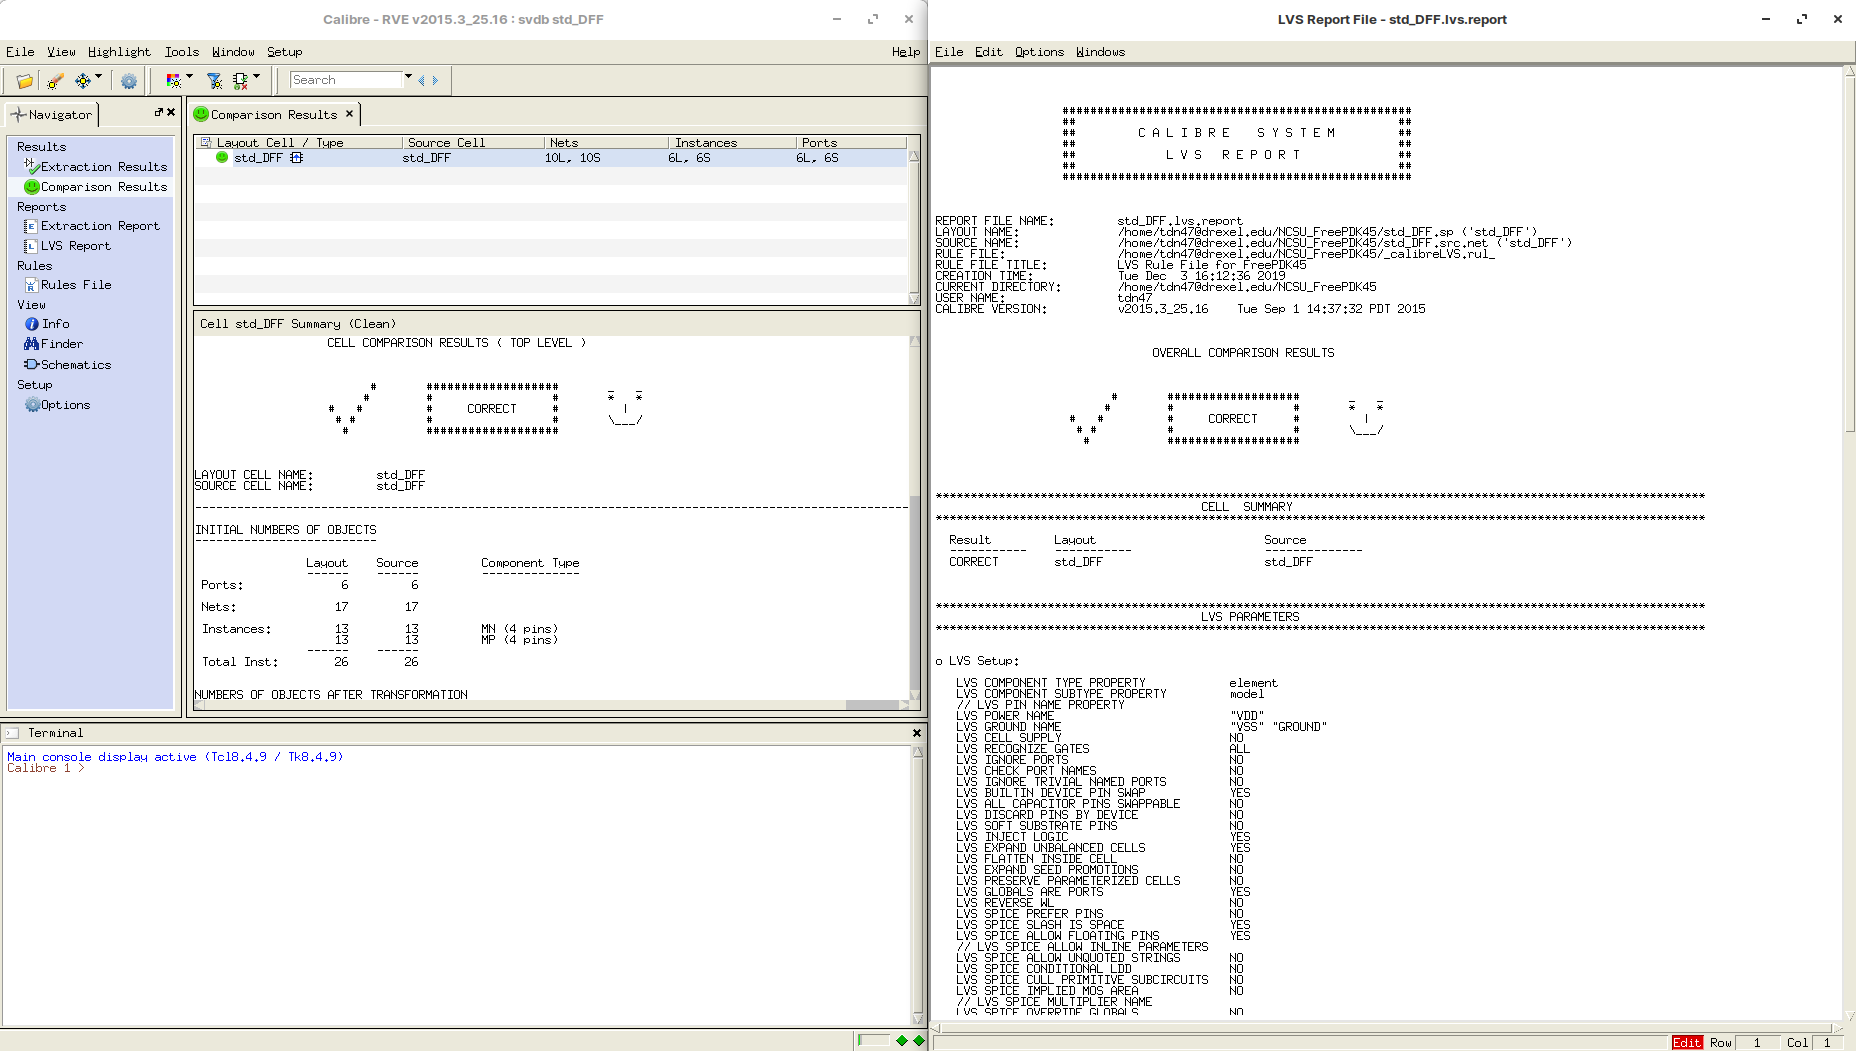
\includegraphics[width=\textwidth]{dff_lvs.png}
%		\caption{DFF's propagation delay}
%		\label{fig9b}
%	\end{subfigure}
%	\caption{Measurements of the DFF's rise/fall time and propagation delay}
%\end{figure}

\end{document}